% Author: Izaak Neutelings (October 2021)
% Inspiration
%   "Very special relativity - An illustrated guide", Sander Bais (2007)
%   http://people.uncw.edu/hermanr/GR/Minkowski/Minkowski.pdf
\documentclass[border=3pt,tikz]{standalone}
\usepackage{amsmath} % for \text
\usepackage{etoolbox} % ifthen
\usepackage[outline]{contour} % glow around text
\usetikzlibrary{calc} % for adding up coordinates
\usetikzlibrary{decorations.markings,decorations.pathmorphing}
\usetikzlibrary{angles,quotes} % for pic (angle labels)
\usetikzlibrary{arrows.meta} % for arrow size
\usepackage{xfp} % higher precision (16 digits?)
\contourlength{1.1pt}

\tikzset{>=latex} % for LaTeX arrow head
\colorlet{myred}{red!85!black}
\colorlet{mydarkred}{red!55!black}
\colorlet{mylightred}{red!85!black!12}
\colorlet{myfieldred}{mydarkred!5} % for S' background
\colorlet{myredhighlight}{myred!20} % highlights simultaneity in ladder paradox
\colorlet{myblue}{blue!80!black}
\colorlet{mydarkblue}{blue!50!black}
\colorlet{mylightblue}{blue!50!black!30}
\colorlet{mylightblue2}{myblue!10}
\colorlet{mygreen}{green!80!black}
\colorlet{mypurple}{blue!40!red!80!black}
\colorlet{mydarkgreen}{green!50!black}
\colorlet{mydarkpurple}{blue!40!red!50!black}
\colorlet{myorange}{orange!40!yellow!95!black}
\colorlet{mydarkorange}{orange!40!yellow!85!black}
\colorlet{mybrown}{brown!20!orange!90!black}
\colorlet{mydarkbrown}{brown!20!orange!55!black}
\colorlet{mypurplehighlight}{mydarkpurple!20} % highlights simultaneity in ladder paradox
\tikzstyle{world line}=[myblue!40,line width=0.3]
\tikzstyle{world line t}=[mypurple!50!myblue!40,line width=0.3]
\tikzstyle{world line'}=[mydarkred!40,line width=0.3]
\tikzstyle{mysmallarr}=[-{Latex[length=3,width=2]},thin]
\tikzstyle{mydashed}=[dash pattern=on 3 off 3]
\tikzstyle{rod}=[mydarkbrown,draw=mydarkbrown,double=mybrown,double distance=2pt,
                 line width=0.2,line cap=round,shorten >=1pt,shorten <=1pt]
%\tikzstyle{rod'}=[rod,draw=mydarkbrown!80!red!85,double=mybrown!80!red!85]
\tikzstyle{vector}=[->,line width=1,line cap=round]
\tikzstyle{vector'}=[vector,shorten >=1.2]
\tikzstyle{particle}=[mygreen,line width=0.9]
\tikzstyle{photon}=[-{Latex[length=5,width=4]},myorange,line width=0.8,decorate,
                    decoration={snake,amplitude=1.0,segment length=5,post length=5}]

\def\tick#1#2{\draw[thick] (#1) ++ (#2:0.06) --++ (#2-180:0.12)}
\def\tickp#1#2{\draw[thick,mydarkred] (#1) ++ (#2:0.06) --++ (#2-180:0.12)}
\def\Nsamples{100} % number samples in plot

\begin{document}


% SPACETIME DIAGRAM - VECTORS
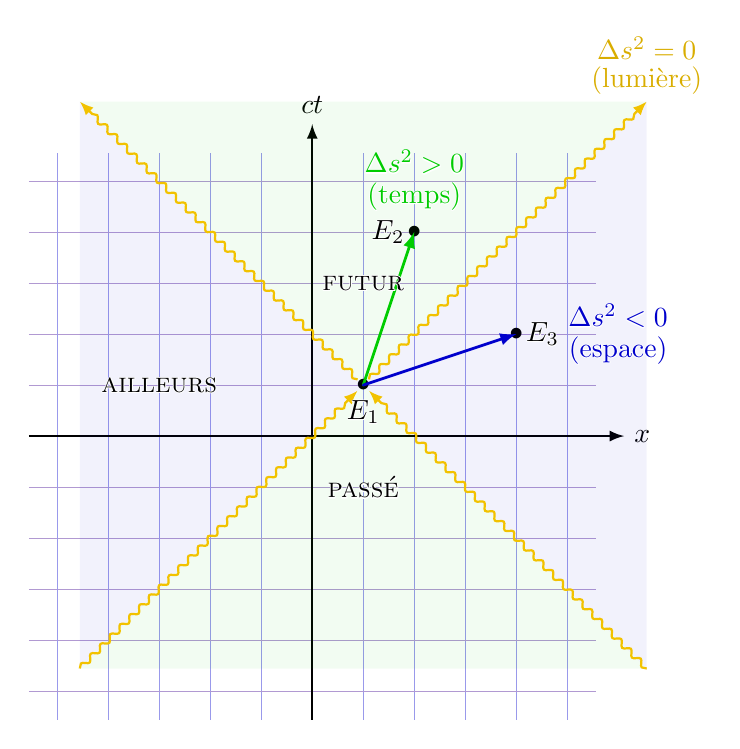
\begin{tikzpicture}[scale=1.8]
  \message{Vectors^^J}
  
  \def\xmax{2}
  \def\xmaxp{2.2} % maximum of rotated axis
  \def\Nlines{5} % number of world lines (at constant x/t)
  \pgfmathsetmacro\d{0.9*\xmax/\Nlines} % grid size
  \pgfmathsetmacro\ang{atan(1/3)} % angle between x and x' axes
  \coordinate (O) at (0,0);
  \coordinate (X) at (\xmax+0.2,0);
  \coordinate (T) at (0,\xmax+0.2);
  \pgfmathsetmacro\xe{\d}
  \pgfmathsetmacro\ye{\d}
  \pgfmathsetmacro\xf{\d}
  \pgfmathsetmacro\yf{3*\d}

  
  % WORLD LINE GRID
  \message{  Making world lines...^^J}
  \foreach \i [evaluate={\x=\i*\d;}] in {1,...,\Nlines}{
    \message{  Running i/N=\i/\Nlines, x=\x...^^J}
    \draw[world line]   (-\x,-\xmax) -- (-\x,\xmax);
    \draw[world line]   ( \x,-\xmax) -- ( \x,\xmax);
    \draw[world line t] (-\xmax,-\x) -- (\xmax,-\x);
    \draw[world line t] (-\xmax, \x) -- (\xmax, \x);
    }
    
    % AXES
    \draw[->,thick] (0,-\xmax) -- (T) node[above] {$ct$};
    \draw[->,thick] (-\xmax,0) -- (X) node[right] {$x$};
    
   
    \node at (\xe,\ye) {$\bullet$};
    \node at (\xe+\xf,\ye+\yf) {$\bullet$};
    \node at (\xe+\yf,\ye+\xf) {$\bullet$};

  \begin{scope}[shift={(\xe,\ye)}]
    
    
    % FILLS
    \fill[myblue,opacity=0.05] % SPACELIKE
    (\xmax,\xmax) -- (-\xmax,-\xmax) -- (-\xmax,\xmax) -- (\xmax,-\xmax) -- cycle;
    \fill[mygreen,opacity=0.05] % TIMELIKE
    (\xmax,\xmax) -- (-\xmax,\xmax) -- (\xmax,-\xmax) -- (-\xmax,-\xmax) -- cycle;
    
    % VECTORS
    \draw[vector,mygreen] (0,0) -- (\xf,\yf)
    node[above=4,align=center]
    { \contour{white}{$\Delta s^2>0$}\\[-1]\contour{white}{(temps)}};
    \draw[vector,myblue] (0,0) -- (\yf,\xf)
    node[right=15,align=center]
    {\contour{white}{$\Delta s^2<0$}\\[-1]\contour{white}{(espace)}};
    % \draw[vector,mygreen,<->] (-2*\d,-\d) --++ (-2*\d,3.5*\d)
    % node[pos=0.8,below left=-2,align=right]
    % {\contour{myblue!5}{timelike}\\[-2]
    % \contour{myblue!5}{separation}\\[-1]
    % \contour{myblue!5}{$\Delta s^2>0$}};
    % \draw[vector,myblue,<->] (2*\d,-\d) --++ (3*\d,-2*\d)
    % node[pos=0.4,above right=-2,align=left]
    % {\contour{myblue!5}{spacelike}\\[-2]
    % \contour{myblue!5}{separation}\\[-1]
    % \contour{myblue!5}{$\Delta s^2<0$}};
    % \draw[vector,myorange,<->] (2*\d,-3*\d) --++ (2*\d,-2*\d)
    % node[pos=0.45,below left=-4,align=center]
    % {\contour{mygreen!5}{lightlike}\\[-2]
    % \contour{mygreen!5}{separation}\\[-1]
    % \contour{mygreen!5}{$\Delta s^2 = 0$}};
    
    % PHOTON
    \draw[photon] ( \xmax,-\xmax) -- ( 0.02*\xmax,-0.02*\xmax);
    \draw[photon] (-\xmax,-\xmax) -- (-0.02*\xmax,-0.02*\xmax);
    \draw[photon] ( 0.02*\xmax,0.02*\xmax) -- ( \xmax,\xmax)
    node[mydarkorange,above=-1,align=center] {$\Delta s ^2 = 0$\\[-2](lumière)};
    \draw[photon] (-0.02*\xmax,0.02*\xmax) -- (-\xmax,\xmax);
  \end{scope}

   \node[below=2] at (\xe,\ye) {\contour{white}{$E_1$}} coordinate (E1);
    \node[left] at (\xe+\xf,\ye+\yf) {\contour{white}{$E_2$}} coordinate (E2);
    \node[right] at (\xe+\yf,\ye+\xf) {\contour{white}{$E_3$}} coordinate (E3);

  \node at (\xe,3*\xe) {\contour{white}{\textsc{futur}}};
  \node[] at (\xe,-\xe) {\contour{white}{\textsc{passé}}};
  \node[] at (-3*\xe,\xe) {\contour{white}{\textsc{ailleurs}}};

  \end{tikzpicture}
  
\end{document}